\section{Parity and the binomial coupling}\label{sec:parity}

We now choose the weight from the polynomial. Parity will convert the
sensitivity problem into the equal-sign edge count of
Lemma~\ref{lem:edges}, while the polynomial degree will produce the
one-sided constraint needed for Lemma~\ref{lem:coupling}.

\begin{proof}[Proof of Theorem~\ref{thm:main}]

We may assume that $p(x)\ne0$ for every $x\in\Omega$.
Indeed, if $p$ takes negative values, add a positive constant smaller than
$\min\{\abs{p(x)}:p(x)<0\}$; otherwise add any positive constant.
Negative values remain negative, while zero values become positive and
positive values stay positive. Thus the perturbation preserves $f$ under
our convention $\sgn(0)=1$, does not increase the degree, and makes $p$
nonzero at every vertex. We henceforth use $p$ for the perturbed polynomial.

Let $\chi=\chi_{[n]}$ be full parity and set
\[
 w=\abs p,\qquad h=\chi f,\qquad q=\chi p.
\]
Full parity changes sign across every edge, so $h(x)=h(y)$ for neighbors
$x,y$ exactly when $f(x)\ne f(y)$. Consequently
\begin{equation}\label{eq:sensitivity-count}
 I(f)=\frac{\abs{\mathcal E_h}}N.
\end{equation}
Here both sides count sensitive edges in both directions.
We have $w>0$ and $hw=q$. Construct the weighted grading
\eqref{eq:grading} from $w$, and let $H$ be multiplication by $h$.
Since $\chi\chi_S=\chi_{[n]\setminus S}$ and $\deg p\le d$, the Fourier
support of $q$ lies in degrees at least $n-d$.

We claim that
\begin{equation}\label{eq:vanishing}
 \Pi_sH\Pi_r=0\qquad\text{if }r+s<n-d.
\end{equation}
To see this, write elements of $E_r\subseteq DV_r$ and $E_s\subseteq DV_s$
as $Da$ and $Db$, with $a\in V_r$ and $b\in V_s$. Then
\[
 \ip{Db}{HDa}=\sum_{x\in\Omega}\overline{b(x)}a(x)w(x)h(x)
 =\sum_{x\in\Omega}\overline{b(x)}a(x)q(x)=0.
\]
The last equality follows from character orthogonality: the product
$\overline b a$ has Fourier degree at most $r+s<n-d$.

Set $T=MH+HM$. Its blocks are
\begin{equation}\label{eq:T-blocks}
 \Pi_sT\Pi_r=(s+r-n)\Pi_sH\Pi_r.
\end{equation}
Thus the anticommutator energy is a weighted second moment of the sum of
the two grade indices:
\[
 \frac1N\norm T_{\HS}^2
 =\sum_{r,s=0}^n(s+r-n)^2\,
   \frac{\norm{\Pi_sH\Pi_r}_{\HS}^2}{N}.
\]
The coefficients on the right define a probability distribution. Indeed,
because $H$ is unitary and the projections are orthogonal,
\[
 \sum_s\norm{\Pi_sH\Pi_r}_{\HS}^2
 =\norm{H\Pi_r}_{\HS}^2=\binom nr.
\]
Decomposing the domain into grades and taking adjoints likewise gives
\[
 \sum_r\norm{\Pi_sH\Pi_r}_{\HS}^2
 =\norm{\Pi_sH}_{\HS}^2
 =\norm{H^*\Pi_s}_{\HS}^2=\binom ns.
\]
Since $\sum_r\binom nr=N$, we may therefore define random indices
$R,S\in\{0,\ldots,n\}$ by
\begin{equation}\label{eq:block-coupling}
 \Prb\{R=r,S=s\}=\frac1N\norm{\Pi_sH\Pi_r}_{\HS}^2.
\end{equation}
Both marginals are $\operatorname{Bin}(n,1/2)$, and the preceding energy
identity becomes
\[
 \frac1N\norm T_{\HS}^2=\E(R+S-n)^2.
\]

To use Lemma~\ref{lem:coupling}, reflect the first index: put $U=S$ and
$V=n-R$. Binomial symmetry gives $U$ and $V$ the same distribution,
with mean $n/2$ and variance $n/4$. Meanwhile,
\eqref{eq:vanishing} gives $R+S\ge n-d$ almost surely, which becomes
$V-U\le d$. Figure~\ref{fig:grade-coupling} shows how the zero-block
region becomes this one-sided support constraint.

\begin{figure}[!htbp]
  \centering
  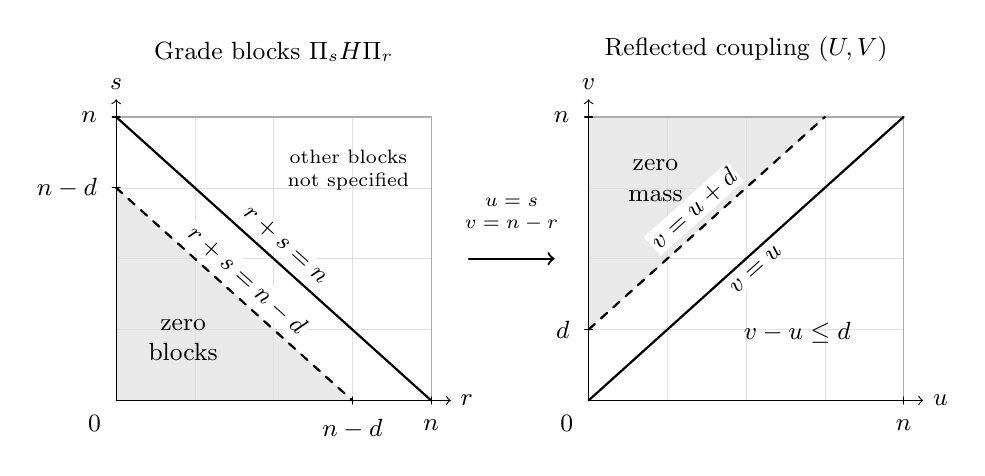
\begin{tikzpicture}[x=1cm,y=.9cm,line cap=round,line join=round,
                      font=\small]
    \begin{scope}
      \fill[gray!17] (0,0) -- (3,0) -- (0,3) -- cycle;
      \draw[step=1,gray!25,very thin] (0,0) grid (4,4);
      \draw[gray!65] (0,4) -- (4,4) -- (4,0);
      \draw[->] (0,0) -- (4.25,0) node[right] {$r$};
      \draw[->] (0,0) -- (0,4.25) node[above] {$s$};
      \node[below left=2pt] at (0,0) {$0$};
      \draw (3,.05) -- (3,-.05) node[below=2pt] {$n-d$};
      \draw (4,.05) -- (4,-.05) node[below=2pt] {$n$};
      \draw (.05,3) -- (-.05,3) node[left=2pt] {$n-d$};
      \draw (.05,4) -- (-.05,4) node[left=2pt] {$n$};
      \draw[thick,dashed] (0,3) -- (3,0)
        node[midway,above=2pt,sloped,fill=white,inner sep=1pt]
        {$r+s=n-d$};
      \draw[thick] (0,4) -- (4,0)
        node[midway,above=2pt,sloped,fill=white,inner sep=1pt]
        {$r+s=n$};
      \node[align=center] at (.85,.85) {zero\\blocks};
      \node[align=center,font=\scriptsize] at (2.95,3.25)
        {other blocks\\not specified};
      \node[above=10pt] at (2,4.25) {Grade blocks $\Pi_sH\Pi_r$};
    \end{scope}

    \draw[->,thick] (4.48,2) -- (5.57,2);
    \node[align=center,font=\scriptsize] at (5.02,2.63)
      {$u=s$\\$v=n-r$};

    \begin{scope}[xshift=6cm]
      \fill[gray!17] (0,1) -- (0,4) -- (3,4) -- cycle;
      \draw[step=1,gray!25,very thin] (0,0) grid (4,4);
      \draw[gray!65] (0,4) -- (4,4) -- (4,0);
      \draw[->] (0,0) -- (4.25,0) node[right] {$u$};
      \draw[->] (0,0) -- (0,4.25) node[above] {$v$};
      \node[below left=2pt] at (0,0) {$0$};
      \draw (4,.05) -- (4,-.05) node[below=2pt] {$n$};
      \draw (.05,1) -- (-.05,1) node[left=2pt] {$d$};
      \draw (.05,4) -- (-.05,4) node[left=2pt] {$n$};
      \draw[thick,dashed] (0,1) -- (3,4)
        node[midway,above=2pt,sloped,fill=white,inner sep=1pt]
        {$v=u+d$};
      \draw[thick] (0,0) -- (4,4)
        node[midway,below=2pt,sloped,fill=white,inner sep=1pt]
        {$v=u$};
      \node[align=center] at (.85,3.1) {zero\\mass};
      \node at (2.65,.95) {$v-u\le d$};
      \node[above=10pt] at (2,4.25) {Reflected coupling $(U,V)$};
    \end{scope}
  \end{tikzpicture}
  \[
    \mathbb P\{R=r,S=s\}
      =2^{-n}\|\Pi_sH\Pi_r\|_{\mathrm{HS}}^2,
    \qquad r+s-n=u-v.
  \]
  \caption{Grade blocks and their reflected coupling, schematic for $0<d<n$.
  Under $U=S$, $V=n-R$, the zero-block region $r+s<n-d$ becomes the
  zero-mass region $v-u>d$, giving $V-U\le d$ almost surely.
  Dashed boundaries are allowed; solid diagonals mark $r+s-n=u-v=0$.
  Each marginal is $\operatorname{Bin}(n,1/2)$. Unshaded locations need
  not carry positive mass, and grid spacing is illustrative.}
  \label{fig:grade-coupling}
\end{figure}


Apply Lemma~\ref{lem:coupling} with $a=d$ and $\sigma=\sqrt n/2$ to obtain
\begin{equation}\label{eq:coupling-bound}
 \frac1N\norm T_{\HS}^2
 =\E(R+S-n)^2=\E(U-V)^2\le4d\sqrt n.
\end{equation}
Finally, \eqref{eq:sensitivity-count} and Lemma~\ref{lem:edges} give
\[
 I(f)=\frac{\abs{\mathcal E_h}}N
 \le\frac2N\norm T_{\HS}^2
 \le8d\sqrt n.
\]
This completes the proof.
\end{proof}


